\chapter{กราฟ (Graph)}

กราฟเป็นหนึ่งในสิ่งที่มีบทบาทมากที่สุดในการเขียนโปรแกรมคอมพิวเตอร์เชิงแข่งขัน (Competitive Programming) เพราะเป็นพื้นฐานสำหรับการพัฒนาต่อยอดความรู้ต่างๆ อีกมากมาย

\section{องค์ประกอบของกราฟ (Component)}

\begin{figure}[h!]
	\centering
    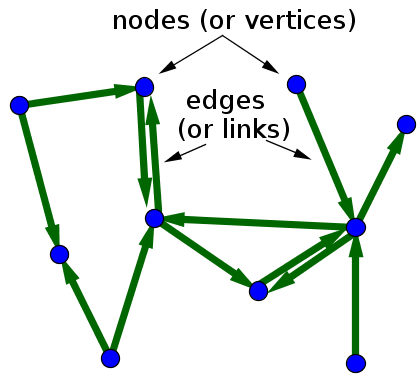
\includegraphics[width=10cm]{images/graph-component}
    \caption{องค์ประกอบของกราฟ}
    \label{fig:graph_component}
\end{figure}


กราฟโดยทั่วไปจะประกอบไปด้วย 2 องค์ประกอบ คือ
\begin{itemize}
\item จุดยอด (Vertices/Nodes)
\item เส้นเชื่อม (Edges/Links)
\end{itemize}

\section{การเก็บกราฟ (Graph Representations)}

การเก็บกราฟ คือการนำองค์ประกอบของกราฟมาเก็บไว้เป็นข้อมูลสำหรับการประมวลผล ซึ่งมี 2 วิธีหลักๆ คือ
\begin{itemize}
\item เมทริกซ์ประชิด (Adjacency Matrix)
\item รายการประชิด (Adjacency List)
\end{itemize}

\subsection{เมทริกซ์ประชิด (Adjacency Matrix)}

วิธีนี้เป็นการเก็บกราฟโดยใช้ Matrix ขนาด $n \times n$ เมื่อ $n$ คือจำนวนจุดยอดทั้งหมดในกราฟ

\begin{figure}[h!]
	\centering
    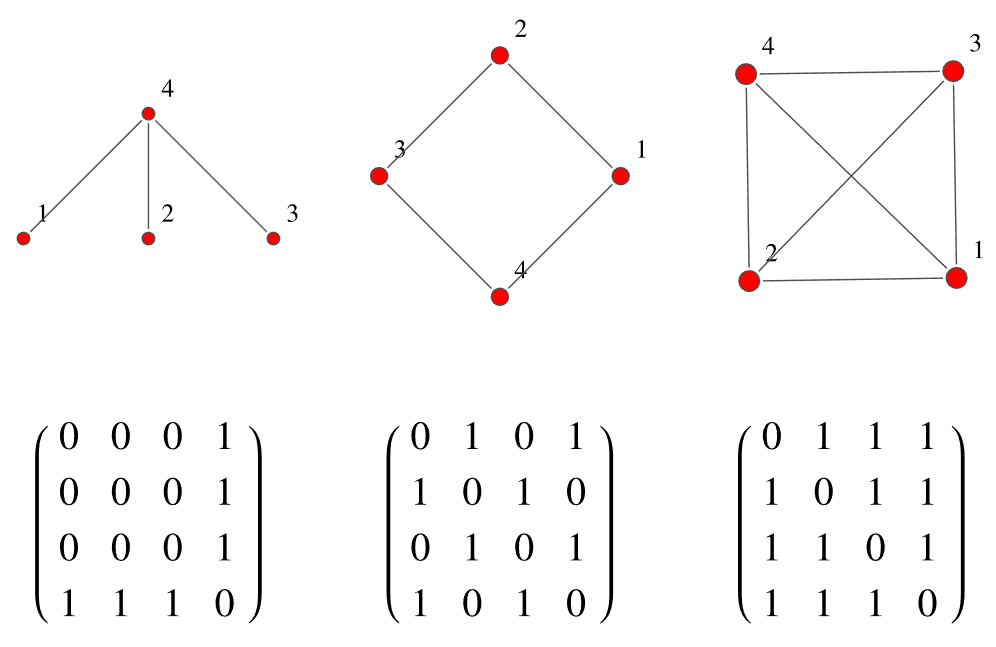
\includegraphics[width=13cm]{images/adjacency-matrix}
	\caption{ตัวอย่างการใช้เมทริกซ์ประชิดกับกราฟที่เส้นเชื่อมไม่มีน้ำหนัก}
    \label{fig:adjacency_matrix}
\end{figure}

เมทริกซ์ที่ใช้อธิบายตัวอย่างข้างต้นนั้นประกอบไปด้วยจำนวน 0 และ 1 เพื่อแทนค่าความจริงของ ``มีเส้นเชื่อมระหว่างจุดยอด $i$  และจุดยอด $j$ เมื่อ $i$ คือแถว และ $j$ คือคอลัมน์''

\newpage

\begin{figure}[h!]
	\centering
    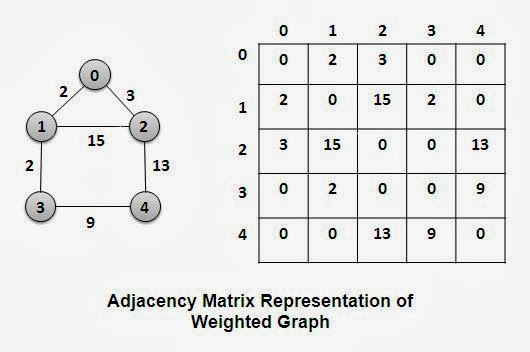
\includegraphics[width=13cm]{images/adjacency-matrix-weighted}
	\caption{ตัวอย่างการใช้เมทริกซ์ประชิดกับกราฟที่เส้นเชื่อมมีน้ำหนัก}
    \label{fig:adjacency_matrix_weighted}
\end{figure}

เมทริกซ์ที่ใช้อธิบายตัวอย่างข้างต้นนั้นเป็นเมทริกซ์ของจำนวนเต็มบวกที่แต่ละจำนวนแทน ``น้ำหนักของเส้นเชื่อมระหว่างจุดยอด $i$  และจุดยอด $j$ เมื่อ $i$ คือแถว และ $j$ คือคอลัมน์''

สำหรับการนำไปเขียนโปรแกรมคอมพิวเตอร์ สามารถนำ array 2 มิติมาใช้แทนเมทริกซ์ 2 มิติได้ โดยมีนิยามแบบเดียวกันกับเมทริกซ์เลย

\begin{lstlisting}
void adjacencyMatrix(int n, int m)
{
	int u, v;
	int matrix[n][n];
	for (int i = 0; i < m; i++){
		scanf("%d %d", &u, &v);
		matrix[u][v] = matrix[v][u] = 1;
	}
}
\end{lstlisting}

\newpage

\subsection{รายการประชิด (Adjacency List)}

วิธีนี้เป็นการเก็บกราฟโดยอาศัยแนวคิดของ Linked list เข้ามาช่วยเก็บข้อมูลว่าปมใดมีเส้นเชื่อมระหว่างกันบ้าง

\begin{figure}[h!]
	\centering
    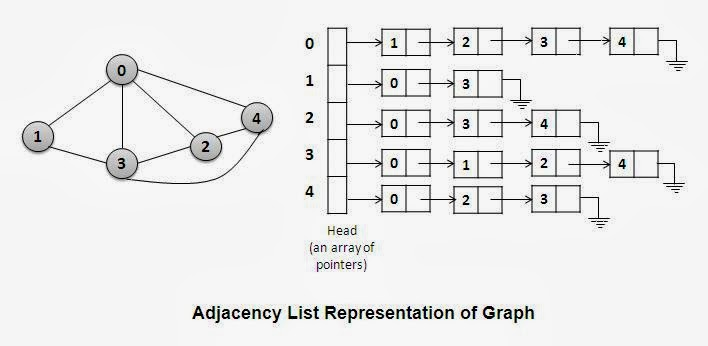
\includegraphics[width=13cm]{images/adjacency-list}
    \caption{ตัวอย่างการใช้รายการประชิด}
    \label{fig:adjacency_list}
\end{figure}

สำหรับการนำไปเขียนโปรแกรมคอมพิวเตอร์ สามารถนำ STL Vector มาใช้ได้

\begin{lstlisting}
void adjacencyList(int n, int m){
	int u, v;
	vector<int> graph[n];
	for (int i = 0; i < m; i++){
		scanf("%d %d", &u, &v);
		graph[u].push_back(v);
		graph[v].push_back(u);
	}
}
\end{lstlisting}